% UC Merced  PhD Dissertation Template
% (UCSD Mathematics Dissertation Template is modified according to the UC Merced guidelines by Lasith Adhikari. Not responsible for any issues regarding modifications. You are welcome to add/update if there is any missing requirernment)
%
% Please read the comments in this file and make appropriate edits.
% NOTE: Always refer to the ``Preperation and Submission Manual for 
% Doctoral Dissertations and Masters Theses for 20**'', where 20** is 
% the year of your graduation, for officiation preparations guidelines.
%
% If you desire more control, please see the attached files:
%   * ucsd.cls -- Class file
%   * uct10.clo, uct11.clo, uct12.clo -- Configuration files for font sizes 10pt,11pt,12pt
%
% CHANGELOG:
%   * Original file adapted from brockman.tex by JRB and RMR
%     to work with ucsd.cls


\documentclass[11pt,oneside,chapterheads]{UCMerced}
% documentclass options: default is 11pt, oneside, final.
% fonts: 10pt, 11pt, 12pt -- are valid for UCSD dissertations (now UC Merced).
% sides: oneside, twoside -- note that two-sided theses are not accepted by OGS
% mode: draft, final -- draft mode switches to single spacing, removes hyperlinks,
%                       and places a black box at every overfull hbox (check these before submission).
% chapterheads -- include this if you want your chapters to read:
% Chapter 1
% Title of Chapter
%
% instead of
%
% 1 Title of Chapter


% Include all packages you need here.  Some standard options are suggested below.

% GEOMETRY - This will force the use of Letter paper.
% Many TeX installations default to A4 paper.  The formatting
% of the thesis class file requires Letter, else the margins
% will be wrong when you go to print it (and OGS will complain).
% If your TeX implementation is not setup for Letter paper, and
% you cannot change it, uncommenting the following line may fix 
% problem.
% \usepackage[paper=letterpaper]{geometry}

\usepackage{graphicx}

%% AMS PACKAGES - Chances are you will want some or all of these if writing a math dissertation.
\usepackage{amsmath, amscd, amssymb, amsthm}
\usepackage{multicol}
\usepackage{tabulary}
\usepackage{tabularx}
\usepackage{makecell}
\usepackage{pgfplots}
\usepackage{longtable}
\usepackage{url}
\usepackage{float}
\usepackage{subcaption}
\usepackage{booktabs}
\usepackage{algorithm}
\usepackage{algorithmic}
\usepackage[Lenny]{fncychap}
\usepackage{pdfpages}
\usepackage{graphbox}

%% LATIN MODERN FONTS (replacements for Computer Modern)
\usepackage{lmodern}
\usepackage[T1]{fontenc}

\usepackage{url}
\usepackage[colorlinks=true, pdfstartview=FitV, linkcolor=black, citecolor=black, urlcolor=black,plainpages=false,pdfpagelabels]{hyperref}
\usepackage{cleveref}
\usepackage[backend=biber,style=apa,sortcites=false,minnames=1,maxnames=3,maxbibnames=4]{biblatex}
\makeatletter
\DeclareCiteCommand{\fullcite}
{\defcounter{maxnames}{\blx@maxbibnames}%
\usebibmacro{prenote}}
{\usedriver
{\DeclareNameAlias{sortname}{default}}
{\thefield{entrytype}}}
{\multicitedelim}
{\usebibmacro{postnote}}
\DeclareCiteCommand{\footfullcite}[\mkbibfootnote]
{\defcounter{maxnames}{\blx@maxbibnames}%
\usebibmacro{prenote}}
{\usedriver
{\DeclareNameAlias{sortname}{default}}
{\thefield{entrytype}}}
{\multicitedelim}
{\usebibmacro{postnote}}
\makeatother

\addbibresource{references.bib}
\let\cite\parencite

\theoremstyle{plain}% default
\newtheorem{theorem}{Theorem}[section]
\newtheorem{lemma}[theorem]{Lemma}
\newtheorem{proposition}[theorem]{Proposition}
\theoremstyle{definition}
\newtheorem{definition}{Definition}[section]

\begin{document}

\title{Fluid Dynamics}
\author{Eunji Yoo}
\degreeyear{2023}
\degree{Doctor of Philosophy}  
\field{Applied Mathematics}

\numberofmembers{4} % |chair|  + |othermembers| (do not count co-chair) % change here
\chair{François Blanchette and Shilpa Khatri}
\memberone{Camille Carvalho}
\membertwo{Chagho Kim}
\memberthree{Ishan Srivastava}
% \memberfour{<COMMITTEE MEMBER 4>}

\begin{frontmatter}
\makefrontmatter % The title, copyright, and signature pages.

\tableofcontents
\listoffigures
\listoftables

%% ACKNOWLEDGEMENTS
\begin{acknowledgements} 
    % Thanks to Francois and Shilpa, 
% \\
% and Michael
\end{acknowledgements}

%% Vita
{
\phantomsection
\addcontentsline{toc}{chapter}{\protect\numberline{}Curriculum Vitae}%
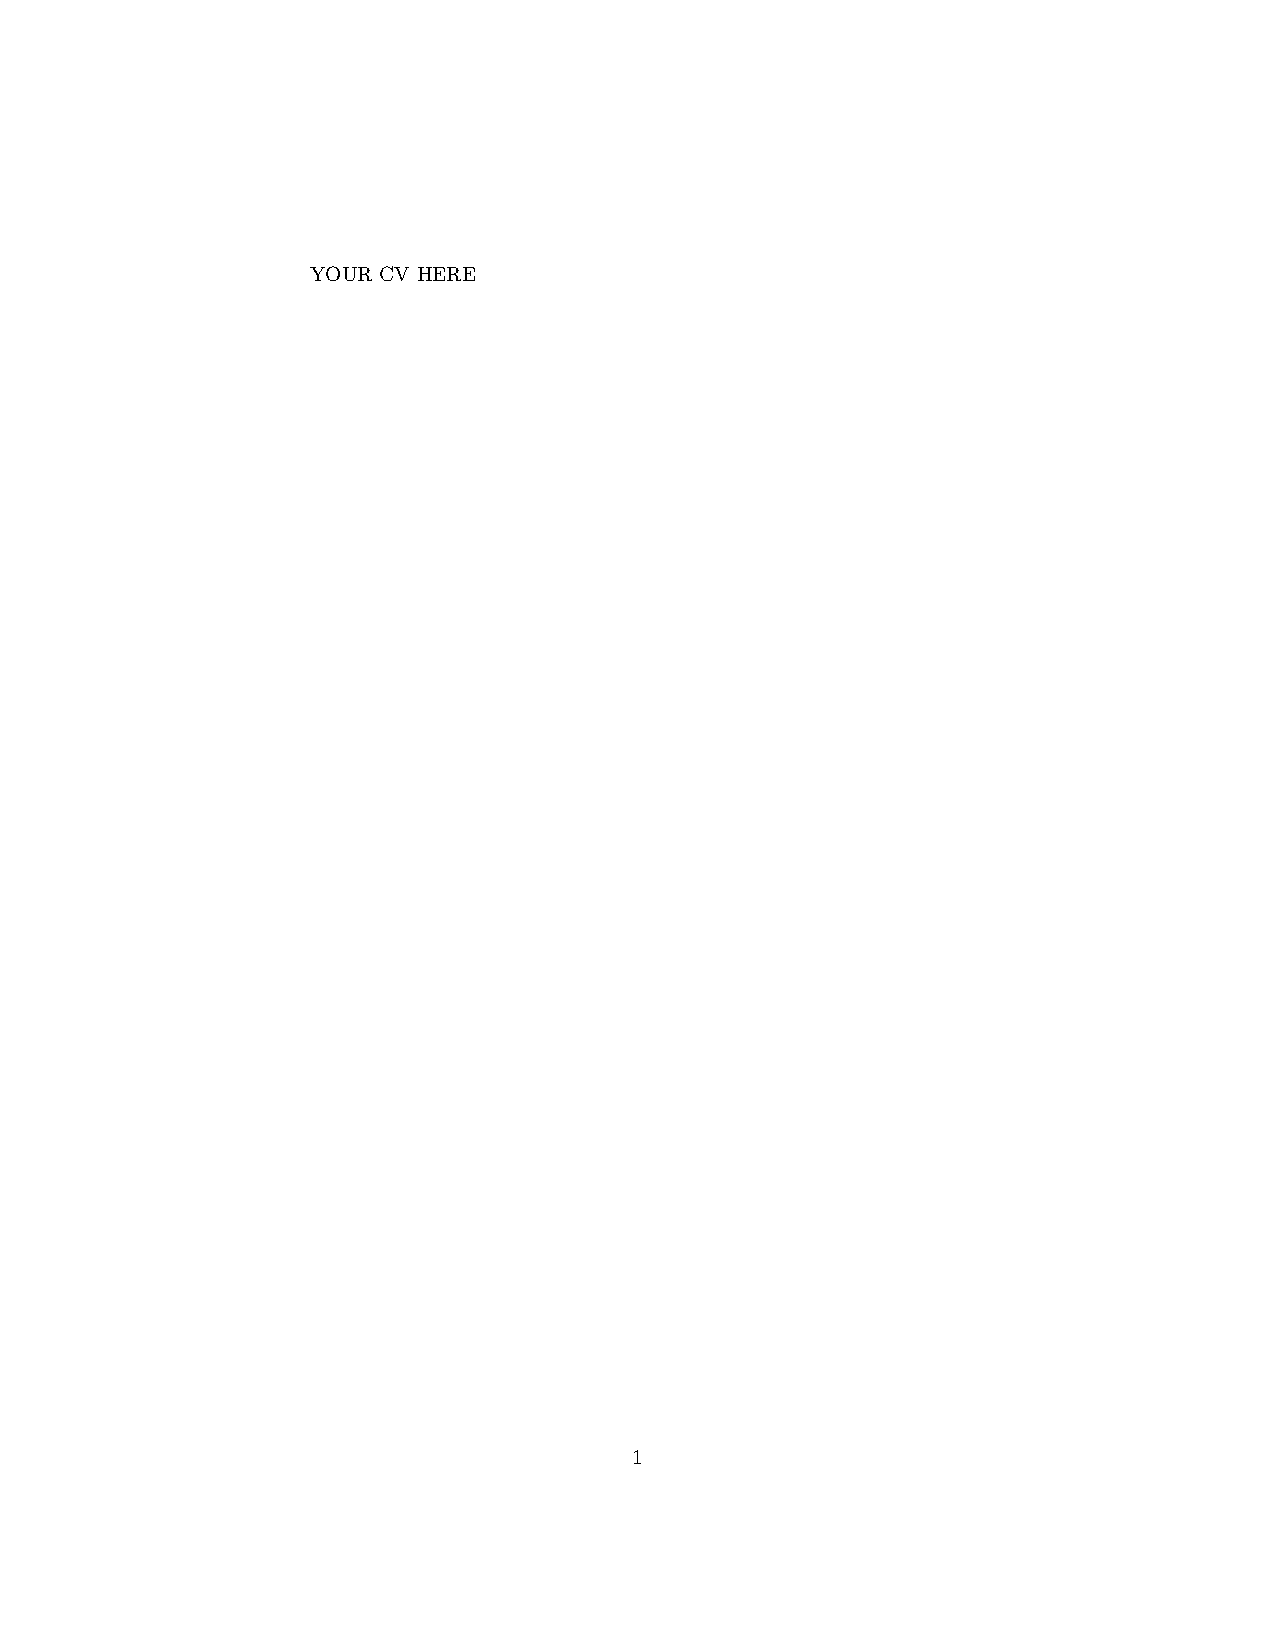
\includepdf[pages=1-,pagecommand={\thispagestyle{preliminary}}]{cv/cv.pdf}
} 

%% Abstract
\begin{abstract}  
    ABSTRACT
\end{abstract}

\end{frontmatter}

%%% DISSERTATION
\chapter{Introduction}
\label{ch:intro}
% INTRODUCTION
Marine aggregates are randomly formed particles composed of organic and inorganic matters, such as phytoplankton, detritus, sediment, and fecal pellets \cite{jackson_simulation_1989}. Since these components stick together arbitrarily, a marine aggregates is often shown a fractal structure. 
These marine aggregates take in carbon dioxide (CO$_2$) during photosynthesis near the surface ocean and carry the dissolved carbon to the deep ocean. 
% The ocean absorbs $40 \%$ of the anthropogenically produced carbon dioxide (CO$_2$) from the atmosphere \cite{omand_sinking_2020}. 
This process removes CO$_2$ from the atmospheric carbon cycle \cite{honjo_understanding_2014}, and plays a role in regulating atmospheric CO$_2$ and climate changes which is one of the most significant environmental problems we face today. 
 \par
 It has been observed that larger sinking aggregates tend to accumulate in thin layers where the ambient fluid is density stratified \cite{alldredge_occurrence_2002}.The highly concentratedthin layers become biological hotspots for bacterial activity and animal feeding. It is ecologically important to understand the marine aggregates dynamics as they delay in settling.
\par
Our research is centered on computing the velocity field around settling marine aggregates and the forces acting on them. We do so using boundary integral equation (BIE) formulations. We construct marine aggregates using cubes to capture their fractal shape, as shown in Figure \ref{fig_cube10}. 
\begin{figure}[ht]
	\begin{center}
		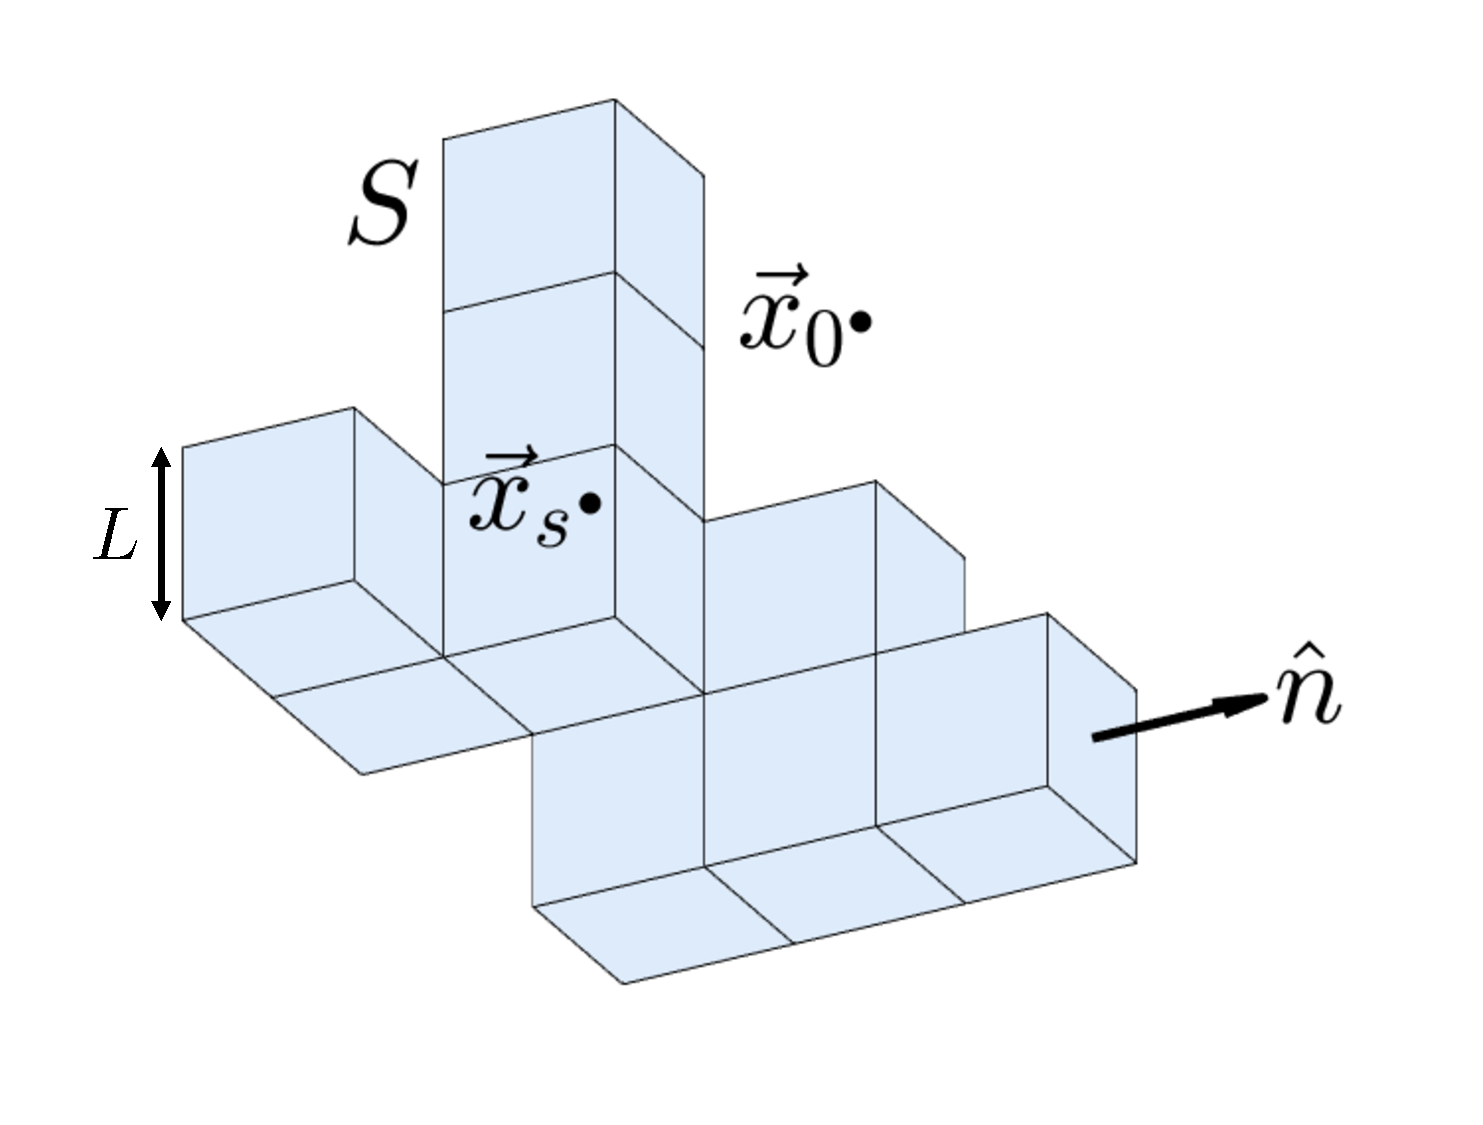
\includegraphics[scale=0.25]{figures/fig_cube10_CC.pdf}
	\end{center}
	\caption{Example aggregate model with 10 cubes. We denote $S$ as the particle surface and $\hat{n}$ as its normal. The vectors $\vec{x}_s$ and $\vec{x}_0$ represent points on and outside of $S$. }
	\label{fig_cube10}
\end{figure}

A detailed explanation of the modeling is in this chapter, section XX.
\par
{\color{red} Move the followings into each subsection.}
In chapter 2, we introduce the governing equations and the velocity solutions to the system. This includes the comparison of two BIE formulations. We then show the numerical methods for solving the velocity field and compuations of forces. We analyze the drag, torque, straining forces acting on the different sizes of aggregates with three types of background flows.
 To simulate concentration dynamics, we couple the velocity obtained using the BIE method with the advection-diffusion equation.
\par
In chapter 3, we consider a varying density fluid case. Due to the fluid density gradient, we modify the fluid momentum equation. We also derive the particular velocity solution in addition to the homogeneous solution. Since the new velocity solution includes a volume integral term which is computationally expensive to evaluate, we use the fast multipole method (FMM). In section XX, we give an introduction to the FMM and its open-source library. 
\par
{\color{blue} ADD DESCRIPTION OF CHAPTER 4 AND 5}
\section{Fluid momentum equations}
To describe the incompressible fluid motion that takes place around marine aggregatess, we consider the Navier-Stokes equations,
\begin{align}
\nabla \cdot \vec{u} = 0 
\label{eq_conserv_mass} \\
\rho 
\left( 
   \frac{\partial \vec{u}}{\partial t} + \vec{u}\cdot \nabla \vec{u}
\right)
  = \nabla \cdot \bar{\bar{\sigma}} +  \rho  \vec{g} ,
\label{eq_momentum_NS}
\end{align}
where $ \rho$ is fluid density (constant) and $\vec{u}, \ \vec{g}$ are fluid velocity and gravity vectors, respectively.
The first equation (\ref{eq_conserv_mass}) shows the conservation of mass and the equation (\ref{eq_momentum_NS}) describes the momentum conservation. 
We also introduce the stress tensor, $\bar{\bar{\sigma}}$ as 
\begin{equation}
   \bar{\bar{\sigma}} = -P \bar{\bar{I}} + {\tilde{\mu}} {\bm D},
   \label{eq_stress_tensor}
\end{equation}
where $P$ is fluid pressure and ${\tilde{\mu}}$ is fluid viscosity. Here, ${\bm D}$ is the symmetric strain rate tensor,
\begin{equation}
   \boldsymbol{D} = \frac{1}{2} \left( \nabla \vec{u} + (\nabla  \vec{u})^T \right).
   \label{eq_strain_rate}
   \end{equation}
Since seawater is Newtonian fluid, following the Newton's law of viscosity, the strain rate (\ref{eq_strain_rate}) becomes $\nabla \vec{u}$. This implies that we can re-write the momentum equation (\ref{eq_momentum_NS}) as
\begin{equation}
  \rho \left( 
   \frac{\partial \vec{u}}{\partial t} + \vec{u}\cdot \nabla \vec{u}
\right)
  = -\nabla P  + {\tilde{\mu}} \nabla^2 \vec{u}+  \rho  \vec{g} 
\end{equation}
For a typical seawater, it is reasonable to say $\rho \approx 1025 \text{kg/m}^3$ and ${\tilde{\mu}} = 1.2 \times 10^{-3}\text{kg}/\text{ms}$.
Also, the gravitaty vector is $\vec{g} = - g\hat{k} \approx -9.8$m/$s^2 \times (0,0,1)$ where $\hat{k}$ points in the vertical direction (upward). 
\par
 The momentum equation (\ref{eq_momentum_NS}) can be linearized for flows where inertial effects are small. 
To estimate the size of the main forces at play, we consider a radius of marine aggregate, $R_a \approx 5 \times 10^{-5}$(m) and the reference Stokes settling speed of an aggregate,
\begin{equation}
    U_s =  \frac{gR_a^2}{{\tilde{\mu}}} (\rho_a-\rho) \approx 3.8 \times 10^{-4} ({\text{m/s}}),
	\label{eq_U_s}
\end{equation}
where $\rho_a \approx 1400\text{kg/m}^3$ is the aggregate mass density. 
When we non-dimensionalize the momentum equation using the length scale, $R_a$ and velocity, $U_s$, we can obtain the following equation:
\begin{equation}
	\left(\frac{\rho U_s R_a}{{\tilde{\mu}}} \right) 
   \left( 
   \frac{\partial \vec{u}'}{\partial t'} + \vec{u}'\cdot \nabla' \vec{u}'
\right)
 = {\nabla'}^2 \vec{u}' - \nabla' P' +  \vec{g}',
 \label{eq_NS_moment_noD}
\end{equation}
where we find and compute the Reynolds number (Re),
\begin{equation}
	\text{Re} = \frac{\rho U_s R_a}{{\tilde{\mu}}} \approx 10^{-2}
	\ll 1.
\end{equation}
Note that we use the prime symbol to represent a dimensionless value.
Since we have fairly small Reynolds number, we may neglect the inertial effects, limiting the left-hand side of equation (\ref{eq_NS_moment_noD}) to zero,
\begin{equation}
   {\nabla'}^2 \vec{u}' - \nabla' P' +  \vec{g}' = 0.
\end{equation}
In this thesis, we therefore consider the following Stokes equations, writing back with dimensions, to describe the fluid flow around the settling aggregates,
 \begin{align}
	\nabla \cdot \vec{u}  = 0  
	% \label{eq_conti2}
	\nonumber \\
	{\tilde{\mu}} \nabla^2 \vec{u}    - \nabla P\ + \rho  \vec{g} = 0.
	\label{eq_stokes2}
\end{align}
The solutions of the system of equations are the fluid velocity, $\vec{u}$, and pressure, $P$. In general, pressure does not induce motion. We see the pressure at rest, denoted as $P_s$, contains the pressure of gravity,  $P_s(\vec{y}) = \rho \vec{g} \cdot \vec{y}$, where $\vec{y} \in \mathbb{R}^3$ is a point in the fluid. Using this static pressure term, we introduce the dynamic pressure $P_d$, defined as 
\begin{equation}
   P_d(\vec{y}) = P(\vec{y}) - P_s(\vec{y}) = P(\vec{y}) - \rho \vec{g} \cdot \vec{y}.
   \label{eq_def_Pd}
\end{equation}
By substituting the expression (\ref{eq_def_Pd}), we obtain
\begin{align}
	\nabla \cdot \vec{u}  = 0  
	% \label{eq_conti2}
	\nonumber \\
	{\tilde{\mu}} \nabla^2 \vec{u}    - \nabla P_d = 0.
	\label{eq_stokes3}
\end{align}
In our simulation, we focus on the velocity field and hydrodynamic forces around the marine aggregate model. 

{\color{red} ADD FIGURE TO EXPLAIN NOTATIONS.}
% {\color{blue}WHY NO PRESSURE?}
%
%===SECTION 2.2=========================================
\section{Boundary integral equation (BIE) formulations} 
For our simulations, we consider a large fluid domain compared to the size of an aggregate, having zero fluid velocity at infinity. We also treat our aggregate surface as a solid. Although marine aggregates are porous, the solid boundary condition is reasonable to apply due to their low permeability. 
% These conditions allow us to eliminate one of the integrals. The detailed derivation is provided in section 2. 
This condition prevents a flow through the aggregate, acting like a solid particle. For this reason, any flow inside of the aggregate is neglected in the remainder of this thesis.  
\par
The fundamental solution $\vec{u}(\vec{y})$, to the Stokes equations, (\ref{eq_stokes2}), at any point $\vec{y} \in \mathbb{R}^3$ that is outside of an object boundary, $S(\vec{x})$, is
% around a solid object is expressed, using the stress vector, $\vec{f}$, 
\begin{equation}
   \vec{u}(\vec{y}) =
	- \frac{1}{8 \pi {\tilde{\mu}}} \int_S  \vec{f}(\vec{x}) \cdot \bar{\bar{G}}(\vec{x},\vec{y}) \ \text{d}S(\vec{x}) 
+ \frac{1}{8 \pi} \int_S
\vec{u}(\vec{x}) \cdot  \bar{\bar{T}}(\vec{x},\vec{y})  
\cdot \hat{n} ( \vec{x})
\ \text{d}S(\vec{x}),
\label{eq_BIE}
\end{equation}
where  $\vec{f}(\vec{x})$ is the stress vector that describes a point force at $\vec{x} \in S$ \cite{pozrikidis_boundary_1992}. Here, the second order tensor in equation (\ref{eq_BIE}) is the Green's function,  $\bar{\bar{G}}(\vec{x},\vec{y})$,
\begin{align}
  \bar{\bar{G}}(\vec{x},\vec{y}) =   
  \frac{\bar{\bar{I}}}{||\vec{x}-\vec{y}||} + \frac{(\vec{x}-\vec{y})(\vec{x}-\vec{y})}{||\vec{x}-\vec{y}||^3},
  \label{eq_stokeslet}
  \end{align}
  and the stress tensor, $\bar{\bar{T}}(\vec{x},\vec{y})$ , associated with the Green's function of the Stokes equations,
  %
  \begin{align}
  \bar{\bar{T}}(\vec{x},\vec{y}) = 
  -6\frac{(\vec{x}-\vec{y})(\vec{x}-\vec{y}) (\vec{x}-\vec{y})}{||\vec{x}-\vec{y}||^5},
  \label{eq_stresslet}
  \end{align}
where $\| \cdot \|$ is the $L^2$ norm. 
Note that $ \bar{\bar{G}}(\vec{x},\vec{y})$ and $ \bar{\bar{T}}(\vec{x},\vec{y}) $ are called  the {\textit{Stokeslet}} and {\textit{Stresslet}}, respectively.
The first integral distribution on the right-hand side of equation (\ref{eq_BIE}) is called the \textit{single-layer potential} and the second one is called the \textit{double-layer potential}. 
\\
{\color{red} ADD THE PHYSICAL MEANING OF THESE TENSORS - FLOW DUE TO A POINT FORCE F}
\par
To compute the velocity at a point on the surface $S$, i.e., $ \vec{x}_s \in S$, we use 
\begin{equation}
   \vec{u}(\vec{x}_s) = - \frac{1}{4 \pi {\tilde{\mu}}} \int_S  \vec{f}(\vec{x}) \cdot \bar{\bar{G}}(\vec{x},\vec{x}_s) \ \text{d}S(\vec{x}) 
+ \frac{1}{4 \pi} 
\int_S
\vec{u}(\vec{x}) \cdot  \bar{\bar{T}}(\vec{x},\vec{x}_s)  
\cdot \hat{n} ( \vec{x})
\ \text{d}S(\vec{x}).
\label{eq_BIE_onS}
\end{equation}
Depending on the fluid domain characteristics and/or type of the object's surface, we can simplify the fundamental equation (\ref{eq_BIE}).


\section{Non-Newtonian fluid}
% Main difference between Newtonian vs Non-Newtonian. Explain the yield stress. Basic idea of rheology, and importnace of the secondary flow we want to capture.
We now turn our attention to a non-Newtonian fluid. This topic is added to my thesis as an extension of one summer internship at the Lawrence Berkeley National Lab in 2022. 
\par
A non-Newtonian fluid shows many interesting behaviors quite different than Newtonian fluids. It has variable viscosity that changes the state of a fluid under a particular pressure, i.e., the viscosity term,${\tilde{\mu}}$ in the stress tensor (\ref{eq_stress_tensor}) is not constant; rahter it is a function of the shear rate ($\dot{\gamma}$), that is
\begin{equation}
   \dot{\gamma} = \left| 
   {\boldsymbol{D}}
   \right|.
\end{equation}
Due to this varying viscosity, the constitutive behavior of non-Newtonian fluids is highly complex. They show intriguing phenomena such as shear thickening, shear thinning, jamming, shear banding, and normal stress differences. This broad class of fluids encompasses various materials of industrial and natural importance, such as granular fluids, polymeric fluids, gels, and suspensions. Complex fluids exhibit two phases as responses to applied stress. This thesis examines the time-dependent coexistence between a fluid's solid and liquid states: the study for this particular fluid type is called {\textit{rheology}}. As the viscosity of a non-Newtonian fluid can be a function of the shear rate, a defining feature of many complex fluids is the presence of yield stress: for an insufficiently stressed material, they behave like an elastic solid, but once the yield stress is exceeded, they flow like a fluid. 
% \begin{figure}[h]
% 	\begin{center}
% 		\includegraphics[scale=0.2]{figures/fig_Rheology_of_time_independent_fluids.pdf}
% 	\end{center}
%    \caption{Rheology graph - need to change}
%     %https://link.springer.com/referenceworkentry/10.1007/978-0-387-92897-5_143 
% 	\label{fig_rheology}
% \end{figure}
\par
Determining one's yield stress is critical to understand rheological behavior accurately. Typically, the stress for a complex fluid can be computed as,
\begin{equation}
   \boldsymbol{\tau} = \mu(\dot{\gamma}) \boldsymbol{D}.
\end{equation}
It was brought to our attention that there are characteristics that could be neglected when we consider the stress linear in $\boldsymbol{D}$. For instance, curvature in free-surface flows, anomalous stress profile in cylindrical Couette flows, or negative rod climbing effect (Weissenberg effect). We thus propose to implement the computational tools to study these secondary flow using the following stress tensor expression:
\begin{align}
  {\bm  \tau}
  =  \ &\mu_1 {\bm D} 
  + \mu_2  \left[ {\bm D}^2  - \frac{\text{tr}\left({\bm D}^2\right)}{3}{\bm I} \right]
  \nonumber \\
  & + \kappa_1 \frac{{\bm D}}{|{\bm D}|} 
  + \kappa_2  \left[ \frac{{\bm D}^2}{|{\bm D}|^2}  
  - \frac{\text{tr}\left({\bm D}^2\right)}{3|{\bm D}|^2}{\bm I} \right].
\end{align}
The terms $\mu_i$ and $\kappa_i$ ($i, j = 1,2,$)coefficients represent the shear rate-dependent and rate-independent contributions, respectively, to the total stress.
\par
With a constitutive rheology code, we can capture such complex continuum hydrodynamics. We thus consider both shear stress rate and the pressure onto the materials of interest as the sources of the yield stress. 
We use AMReX framework, developed at LBNL, NREL, and ANL, to solve flow motion. We implement the granular material viscosity computation in \verb+incflo+, which is an AMReX-based code for modeling the variable density incompressible Navier-Stokes equations without subcycling in time.





\chapter{Chapter 2}
Chapter 2

%% Add more chapters here if necessary

\chapter{Conclusion and future work}
\label{ch:conclusion}
CONCLUSION 

%% BIBLIOGRAPHY
\addcontentsline{toc}{chapter}{Bibliography}
\printbibliography

%% APPENDIX
\appendix
\chapter{Appendix for chap 2}

\section{Exact Kernel Integration}
\label{appdx}

% \begin{figure}[ht]
% 	\begin{center}
% 		\epsfig{figure=./figures/fig_appendix.pdf,height=5cm}
% 	\end{center}
% 	\caption{Schematic of the mapped domain where numerical integration is performed.}
% 	\label{fig_appdx}
% \end{figure}

\begin{figure}[ht]

	\begin{center}
		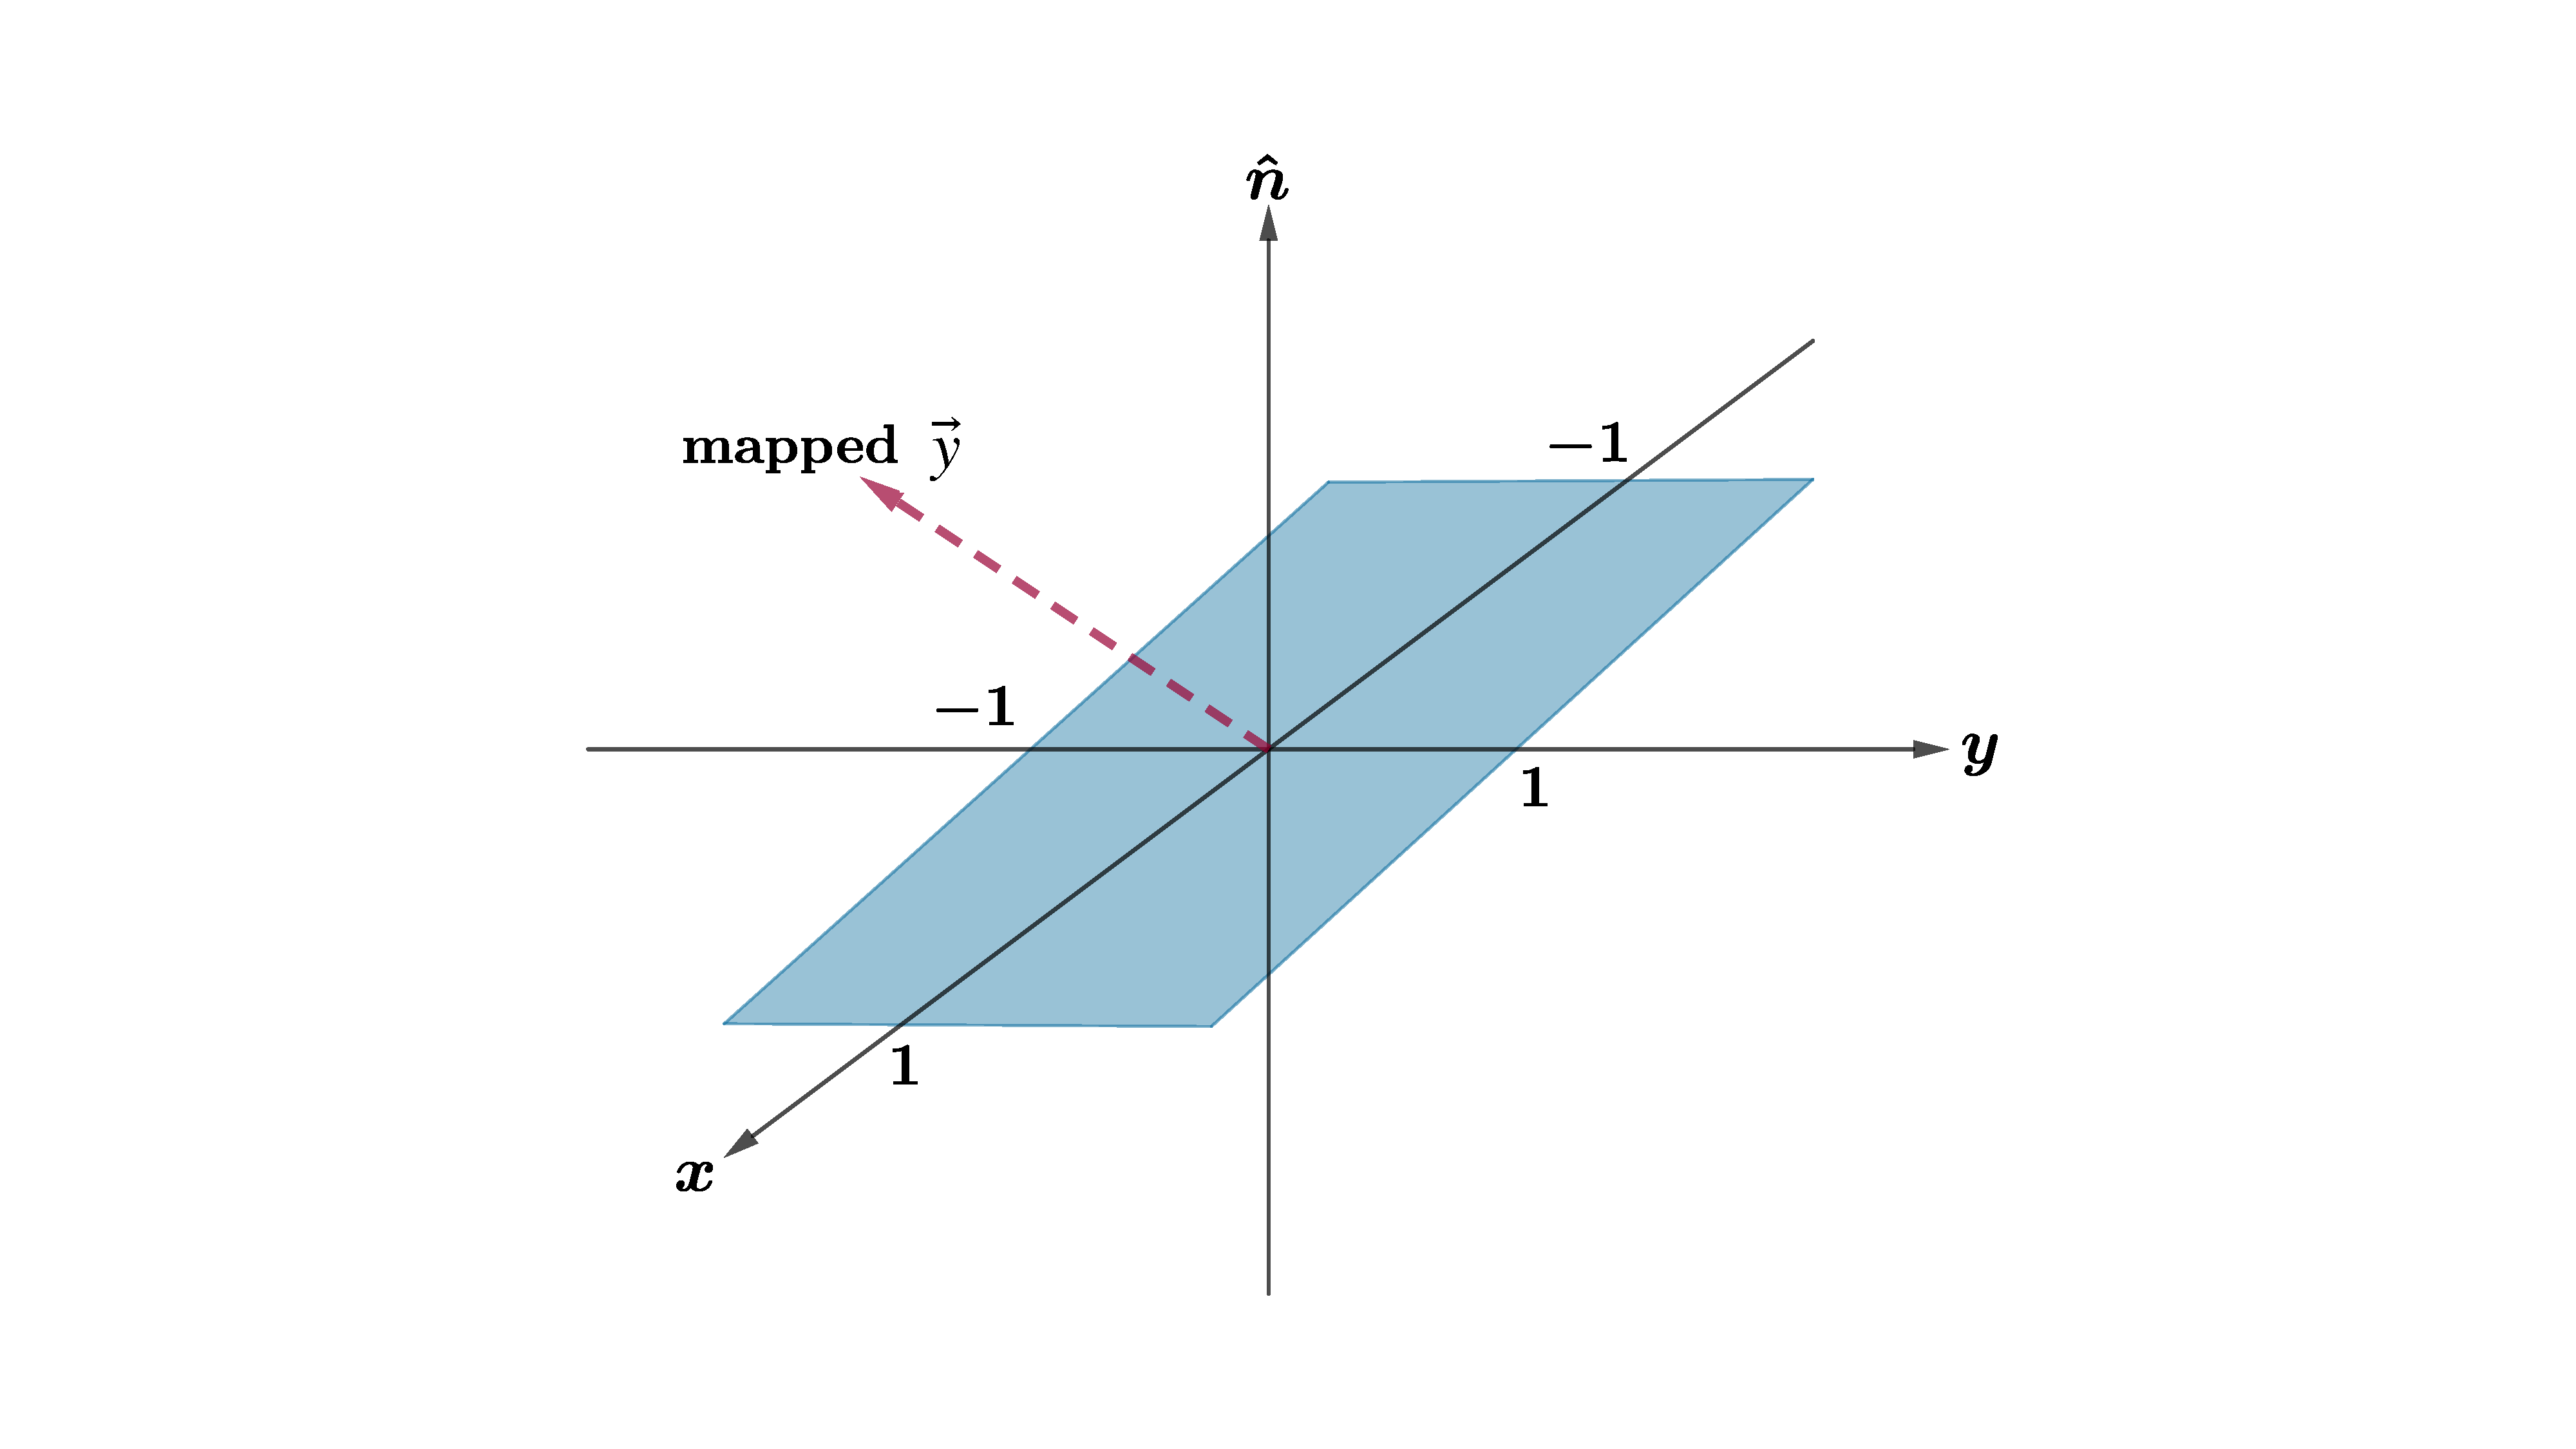
\includegraphics[scale=0.25]{figures/fig_appendix.pdf}

	\caption{Schematic of the mapped domain where numerical integration is performed.} 

\label{fig_appdx}
\end{center}
\end{figure}

When computing the flow around the aggregates, we need to integrate over square surfaces. 
To integrate over any square face, we first map the square over which we need to integrate to the square $(x,y,0)$ with $x \in [-1,1]$ and $y \in  [-1,1]$, as depicted in Fig. (\ref{fig_appdx}). The normal to the surface is thus always in the $z-$direction. We may then exactly evaluate all the surface integrals involved in either the single-layer or double-layer potential methods. 


\subsection{Single-layer potential}
\label{appdx_single}

In the single-layer potential approach, we need to compute integrals of the form
\begin{align}
 \int_S  \left( \frac{\bar{\bar{I}}}{  ||\vec{x}-\vec{y} ||  } + \frac{(\vec{x}-\vec{y}) (\vec{x}-\vec{y}) }{||\vec{x}-\vec{y}||^3} \right)  \ \text{d}S(\vec{x})
 \nonumber \\
 = \int_S   \frac{\bar{\bar{I}}}{  ||\vec{x}-\vec{y} ||  }\text{d}S(\vec{x}) + \int_S   \frac{(\vec{x}-\vec{y}) (\vec{x}-\vec{y}) }{||\vec{x}-\vec{y}||^3}   \text{d}S(\vec{x}) 
 = I_1 + I_2
 \label{eq_slp_int}.
\end{align}
Here, we have that $ \vec{x} = (x,y,0)$ and we write $\vec{y}= (x_0,y_0,z_0)$ and
\[
 ||\vec{x}-\vec{y}||=R(x,y) = \sqrt{ (x-x_0)^2+(y-y_0)^2+z_0^2  }
\]
 We first consider the case when $x_0=y_0=z_0=0$, which arises when integrating over a face centered at the point where we are computing the velocity. In that case, we have $R(x,y) = \sqrt{x^2+y^2}$. We find for the diagonal terms of $I_1$
\begin{equation}
\int_{-1}^{1} \int_{-1}^{1} \frac{1}{   \sqrt{ x^2+y^2  }  }  \ \text{d}x \text{d}y = 8 \ \text{arcsinh}(1)
\end{equation}
and all the non-diagonal terms are zero. 

Away from the singularity, we can generally find antiderivatives computed using Mathematica. For the integral $I_1$, we have
\begin{align}
\int_S \frac{1}{||\vec{x}-\vec{y}||}  \text{d}S(\vec{x})
 =
\int_{-1}^1 \int_{-1}^1  \frac{1   }{R(x,y)  } \ \text{d}x \text{d}y
\nonumber \\
=
(x-x_0) \log \left(R(x,y) + (y-y_0)\right)
+(y-y_0)\log \left(R(x,y) +(x-x_0)   \right) \nonumber \\
\left. \left. -z_0 \arctan \left(\frac{(x-x_0) (y-y_0)}{z_0 R(x,y) }\right)
+z_0 \arctan \left(\frac{(y-y_0)}{z_0}\right)
-(y-y_0)\right|_{x=-1}^1 \right|_{y=-1}^1 .
\label{eq_slp_const}
\end{align}

Note that there is no issue with evaluating the arctangent when $z_0=0$, as the multiplication by $z_0$ yields zero. Also, we need to be careful using this antiderivative when evaluating cases where $z_0=0$ and  $|x_0| = |y_0|=1$. In that case, the integral simplifies to 
\begin{equation}
\int_{-1}^{1} \int_{-1}^{1} \frac{1}{   \sqrt{ 1+x^2  }  }  \ \text{d}x \text{d}y = 4 \sinh^{-1}(1).
\end{equation}

Next, we consider the second part of the integral equation (\ref{eq_slp_int}), $I_2$, which we index with $m$ and $n$
\begin{equation}
I_2 = \int_{-1}^1  \int_{-1}^1  \frac{(\vec{x}-\vec{y})_m (\vec{x}-\vec{y})_n }{R(x,y)^3}
	\ \text{d}x \text{d}y
.
\label{eq_slp_xx}
\end{equation}
Note that the numerator in equation (\ref{eq_slp_xx}), written in index notation,  refers to four different cases. There are two square-like terms
\begin{equation*}
\text{(a)} ~~~	(x-x_0)(x-x_0) ~~~ \text{or} ~~~	(y-y_0)(y-y_0)
	  ~~~\text{and (b)} ~~~ 	z_0^2,
\end{equation*}
and two mixed terms
\begin{equation*}
\text{(c)} ~~~	(x-x_0)(y-y_0)
	 ~~~ 	\text{and (d)} ~~~-(x-x_0)(z_0)
	 ~~~ \text{or} ~~~	-(y-y_0)(z_0).
\end{equation*}

Again, we treat $x_0=y_0=z_0=0$ separately. The first two diagonal terms (case (a)) are then
\begin{equation}
	\int _{-1}^1\int _{-1}^1
	\frac{x^2}{\left(x^2+y^2\right)^{3/2}}
	\ \text{d}x \text{d}y
	=4 \ \text{arcsinh}(1).
\end{equation}
The third diagonal term is zero because of $z_0=0$, and every non-diagonal term is zero by symmetry.

Assuming that $x_0y_0z_0\neq0$,  we consider cases (a)-(d) in turn.
For case (a), we have
\begin{align}
\int_{-1}^1 \int_{-1}^1 \frac{(x-x_0)^2 }{R(x,y)^{3}}  \ \text{d}x \text{d}y
=(y-y_0) \left(\log \left(R(x,y)+x\right)-1\right) \nonumber \\ 
 +z_0  \arctan\left(\frac{(y-y_0)}{z_0}\right) \left. \left.
-z_0 \arctan\left(\frac{(x-x_0)(y-y_0)}{ z_0R(x,y)}\right) \right|_{x=-1}^1 \right|_{y=-1}^1 .
\label{eq_slp_int_xx}
\end{align}
This case does not have evaluation issues since the argument of the logarithm can only be zero if $y=y_0$, which causes this entire term to be zero. Also, $R(x,y)$ can only be zero if $z_0=0$, which would then ensure that the third term would be zero. 
Note that the cases with numerator $(y-y_0)^2$ and  $(x-x_0)^2$ are equivalent if we swap the $x$ and $y$ variables by choosing a different mapping.


Case (b) is simpler since the $z_0$ term is constant. 
\begin{align}
\int_{-1}^1 \int_{-1}^1 \frac{z_0^2 }{R(x,y)^{3}}  \ \text{d}x \text{d}y
&= \left. \left.
z_0  \arctan \left(\frac{(x-x_0) (y-y_0)}{z_0  R(x,y)  }\right) \right|_{x=-1}^1 \right|_{y=-1}^1 
\label{eq_slp_int_zz}
\end{align}
Here, the only possibility to have an undefined value is when $z_0=0$, which simply gives a value of zero as the multiplying factor $z_0$ dominates the arctangent.


For case (c), we find
\begin{equation}
\int _{-1}^1\int _{-1}^1
\frac{(x-x_0)(y-y_0) }{R(x,y)^{3}}  \ \text{d}x \text{d}y
= \left. \left.
-R(x,y) \right|_{x=-1}^1 \right|_{y=-1}^1 .
\label{eq_slp_int_xy}
\end{equation}


Finally, for case (d), we have
\begin{equation}
\int_{-1}^1 \int_{-1}^1 \frac{(x-x_0) z_0 }{R(x,y)^{3}}  \ \text{d}x \text{d}y
= \left. \left.
-z_0 \log \left( R(x,y)+  (y-y_0)   \right) \ \right|_{x=-1}^1 \right|_{y=-1}^1 .
\label{eq_slp_int_xz}
\end{equation}
As before, this case also does not have any issue since $R(x,y)+(y-y_0)$ can only be zero if $z_0=0$, which causes the entire term to be zero.  

\subsection{Double-layer potential}

We now consider the double-layer potential integrals of the form
\begin{equation}
 \int_S
 \frac{(\vec{x}-\vec{y})(\vec{x}-\vec{y})     }{R(x,y)^5 }
\ (\vec{x}-\vec{y}) \cdot  n_k    \ \text{d}S(\vec{x}).
\label{eq_dlp_int}
\end{equation}
Since the inner product between the position and normal vectors always gives $z_0$ in the mapped coordinates, we focus on the integral,
\begin{equation}
\int_S
 \frac{(\vec{x}-\vec{y})_m(\vec{x}-\vec{y})_n     }{R(x,y)^5 }
    \ \text{d}S(\vec{x}).
\label{eq_dlp_int2}
\end{equation}
Note that we only need to compute this integral when $z_0\neq 0$, as otherwise equation (\ref{eq_dlp_int})  is zero because of the inner product. This also implies that $R(x,y)$ may never be zero.


We now consider the following four cases: \\ (a) $m=n=1$ or $m=n=2$, \\ (b) $m=n=3$, \\ (c) $m=1$, $n=2$ or $m=2$, $n=1$, \\ (d) $m=$1 or 2 and $n=3$, or $m=3$ and $n=$1 or 2 vice versa. 

For case (a), we find
\begin{align}
  \int_{-1}^1 \int_{-1}^1
  \frac{ (x-x_0)^2 }{R(x,y)^5 }
  \ \text{d}x \text{d}y
  \nonumber \\
  =
  \frac{1}{3} 
  \biggl[
  \frac{1}{z_0}\arctan \left(\frac{(x-x_0)(y-y_0)}{z_0 R(x,y)}\right) \biggr.
  \left. \left. \biggl. -\frac{(x-x_0) (y-y_0)}{\left((x-x_0)^2+z_0^2\right) R(x,y)}
  \biggr]   \ \right|_{x=-1}^1 \right|_{y=-1}^1 .
\label{eq_dlp_int_xx}
\end{align}
Since $z_0\neq0$ and $R(x,y) \neq 0$, there are no issues when evaluating this antiderivative. 

For case (b),
\begin{align}
\int_{-1}^1 \int_{-1}^1
\frac{ z_0^2     }{R(x,y)^5 }
\ \text{d}x \text{d}y
=
\frac{1}{3}
\biggl[
\frac{1}{z_0}
\arctan \left(\frac{(x-x_0) (y-y_0)}{z_0 R(x,y)}\right)
\nonumber \\
 \left. \left. +\frac{(x-x_0) (y-y_0) \left(R(x,y)^2+ z_0^2\right)}{\left((x-x_0)^2+z_0^2\right) \left((y-y_0)^2+z_0^2\right) R(x,y)}
\biggr] \right|_{x=-1}^1 \right|_{y=-1}^1 ,
\label{eq_dlp_int_zz}
\end{align}
which again can always be evaluated directly when $z_0\neq0$.


Case (c) is relatively simple, as we can see, 
\begin{equation}
\int_{-1}^1 \int_{-1}^1
\frac{ (x-x_0)(y-y_0)    }{R(x,y)^5 }
\ \text{d}x \text{d}y
= \left. \left.
\frac{1}{3 R(x,y)} \right|_{x=-1}^1 \right|_{y=-1}^1 .
\label{eq_dlp_int_xy}
\end{equation}


Finally, case (d) is 
\begin{equation}
\int_{-1}^1 \int_{-1}^1
\frac{ (x-x_0)z_0    }{R(x,y)^5 }
\ \text{d}x \text{d}y
= \left. \left.
-\frac{(y-y_0) z_0}{3 \left((x-x_0)^2+z_0^2\right) R(x,y)} \right|_{x=-1}^1 \right|_{y=-1}^1.
\label{eq_dlp_int_xz}
\end{equation}
Once again, this is simple to evaluate when $z_0\neq0$.


\section{Extensional Flow past a Sphere}


In the case of a sphere of radius $R_s$, one may compute an exact solution for the flow satisfying $\vec{U}_{bg} = \bar{\bar{M}}\cdot \vec{x}$ at infinity and $\vec{U}_{bg} = 0$ on the surface of the sphere. 

The Stokes flow around the sphere is then \cite{guazzelli_physical_2011}
\[
\vec{u} = \left( \bar{\bar{M}} \cdot \vec{x} \right) \left( 1 - \frac{R_s^5}{r^5} \right) + \left( (\bar{\bar{M}} : \vec{x} \vec{x}) \vec{x} \right) \ \left( \frac{5}{2} \right)\left( \frac{R_s^5}{r^7}- \frac{R_s^3}{r^5} \right)
\]
and the corresponding pressure is
\[
P = - 5 \mu R_s^3  \frac{\bar{\bar{M}} : \vec{x}\vec{x}}{r^5}
\]
where $\vec{x}$ is the position vector and $r$ the distance to the center of the sphere. The stress tensor is then
\begin{eqnarray*}
\bar{\bar{T}} &=&  5 \mu R_s^3  \frac{\bar{\bar{M}} : \vec{x}\vec{x}}{r^5} + 2 \bar{\bar{M}} \left( 1 - \frac{R_s^5}{r^5} \right).+ ( \vec{x} (\bar{\bar{M}} \cdot \vec{x})  +  (\bar{\bar{M}} \cdot \vec{x}) \vec{x} ) \left( \frac{10R_s^5}{r^7} - \frac{5R_s^3}{r^5} \right)  \\
& & + 5 \left( \frac{R_s^5}{r^7}- \frac{R_s^3}{r^5} \right) (\bar{\bar{M}} : \vec{x}\vec{x}) \bar{\bar{I}} +  5 \left( \frac{5R_s^3}{r^7}- \frac{7R_s^5}{r^9} \right) (\bar{\bar{M}} : \vec{x}\vec{x}) \vec{x} \vec{x}
\end{eqnarray*}

On the surface of the sphere, where $r=R_s$, we consider the stress vector, $\vec{f} = \bar{\bar{T}}\cdot \hat{n}$, where $\hat{n} = \vec{x}/R_s$, and find
\[
\vec{f} = \left.  \bar{\bar{T}} \cdot \hat{n} \right|_{r=R_s}  = \frac{5 \mu}{R_s^2} \left( \frac{2 \bar{\bar{M}}: \vec{x} \vec{x}}{R_s} -  \frac{2 \bar{\bar{M}}: \vec{x} \vec{x}}{R_s} + \bar{\bar{M}} \cdot \vec{x} R_s  \right) = \frac{5 \mu \bar{\bar{M}} \cdot \vec{x}}{R_s}
\]

For an eigenvector $\hat{v}_i$ with eigenvalue $\lambda_i$, we thus find
\[
S_i  = \frac{1}{2} \int_S | \vec{f} \cdot \vec{v}_i | \ dS = 5  \pi \mu R_s^2 \lambda_i .
\]



\end{document}

